\chapter{Análise Estatística Não Paramétrica}
\label{chap:analise_estatistica_np}

Tendo em vista que os dados das métricas de conectividade (diferença entre Pós e Pré) não se comportam de maneira normal (ver Capítulo~\ref{chap:analise_distribuicao_normalidade}), optamos por empregar testes estatísticos não paramétricos para comparar as condições de estimulação (\texorpdfstring{\textit{cathodic} versus \textit{sham}}{cathodic versus sham}). Essa escolha evita pressupostos inadequados sobre a distribuição dos dados e confere maior robustez às inferências.

Nesta etapa, foram aplicados os seguintes testes:
\begin{itemize}
    \item \textbf{Mann-Whitney U:} Teste para amostras independentes, comparando as condições para cada faixa de frequência e grupo de canais. O efeito foi estimado pela fórmula:
    \[
    \text{effect size} = \frac{2\cdot \text{stat}}{n_{\text{cathodic}} \cdot n_{\text{sham}}} - 1.
    \]
    \item \textbf{Wilcoxon:} Teste para amostras pareadas, no qual os dados foram emparelhados por atleta, par de canais e faixa de frequência, possibilitando uma comparação intraindividual entre as condições.
    \item \textbf{Kruskal-Wallis:} Teste para múltiplos grupos, empregado para comparar as condições quando os dados foram agrupados por faixa de frequência, com o tamanho do efeito estimado pela razão entre a estatística do teste e o número total de observações menos um.
\end{itemize}

Os testes foram realizados separadamente para cada uma das métricas de conectividade 
(\texttt{median\_plv\_diff}, \texttt{median\_pli\_diff} e \texttt{median\_cf\_plm\_diff}) 
e para os dois grupos de canais: \texttt{EEG\_EEG} e \texttt{EEG\_ECG}. 

Ressalta-se que, embora o código inclua procedimentos para remoção de dados nulos, 
na prática, esses valores não estão presentes, servindo apenas para tratamento de exceções.

\section{Resultados dos Testes}

\subsection{\texorpdfstring{Métricas para \texttt{median\_pli\_diff}}{Métricas para median\_pli\_diff}}

\paragraph{Grupo EEG\_EEG:}
\begin{itemize}
    \item \textbf{Mann-Whitney U:} As faixas \emph{alpha, delta, gamma} e \emph{theta} apresentaram diferenças significativas (p-valores $< 0.001$), enquanto a faixa \emph{beta} teve um resultado marginal ($p \approx 0.051$).
    \item \textbf{Wilcoxon:} Os testes pareados indicaram significância robusta em todas as faixas, com tamanho de efeito em torno de $0.477$.
    \item \textbf{Kruskal-Wallis:} As faixas \emph{alpha, delta, gamma} e \emph{theta} foram significativamente diferentes, com \emph{beta} sendo marginalmente não significativa.
\end{itemize}

\subsection{\texorpdfstring{Métricas para \texttt{median\_cf\_plm\_diff}}{Métricas para median\_cf\_plm\_diff}}

\paragraph{Grupo EEG\_ECG:}
\begin{itemize}
    \item \textbf{Mann-Whitney U:} Foram significativas as faixas \emph{alpha, beta} e \emph{delta} (p-valores menores que 0.05), enquanto \emph{gamma} e \emph{theta} não apresentaram significância.
    \item \textbf{Wilcoxon:} Todos os testes resultaram em p-valores extremamente baixos, com tamanhos de efeito de aproximadamente $0.358$.
    \item \textbf{Kruskal-Wallis:} As faixas \emph{alpha, beta} e \emph{gamma} foram significativas, mas \emph{delta} e \emph{theta} não apresentaram diferenças estatísticas.
\end{itemize}

\section{Discussão e Justificativa dos Métodos}

Dado que os testes de normalidade indicaram violações significativas do pressuposto de normalidade para as métricas analisadas, a utilização de testes não paramétricos se mostrou necessária. Tais métodos não dependem de pressupostos sobre a distribuição dos dados, oferecendo uma análise mais robusta e confiável. Além disso, a aplicação de múltiplos testes (Mann-Whitney U, Wilcoxon e Kruskal-Wallis) permitiu uma avaliação abrangente das diferenças entre as condições \texorpdfstring{\texttt{cathodic}}{cathodic} e \texorpdfstring{\texttt{sham}}{sham}, considerando tanto comparações entre grupos independentes quanto análises pareadas intraindividuais.

Os resultados indicam que, para a maioria das faixas de frequência e para as métricas \texorpdfstring{\texttt{median\_pli\_diff}}{median_pli_diff} e \texorpdfstring{\texttt{median\_cf\_plm\_diff}}{median_cf_plm_diff}, existem diferenças estatisticamente significativas entre as condições, reforçando a importância da modulação induzida pela estimulação. Por sua vez, os achados para \texorpdfstring{\texttt{median\_pli\_diff}}{median_pli_diff} foram menos consistentes, variando conforme o teste e a faixa considerada.

Em suma, a escolha dos testes não paramétricos foi justificada pela distribuição não normal dos dados, e os resultados obtidos fornecem evidências sólidas de diferenças na sincronização de fase entre as condições experimentais, reforçando os efeitos da estimulação no contexto das análises de conectividade.

\section{Detecção de Outliers, Análise Bootstrap e Correções para Comparações Múltiplas}

Para aprimorar a qualidade dos dados e reduzir o impacto de pontos atípicos nas análises subsequentes, executamos uma etapa de detecção e remoção de outliers utilizando o método ECOD (Empirical Cumulative Distribution-based Outlier Detection). Esse método é especialmente adequado para nosso conjunto de dados por sua natureza não paramétrica, que permite identificar anomalias sem pressupor uma distribuição específica. O ECOD estima a função de distribuição cumulativa empírica em cada dimensão, identificando como outliers os pontos que se desviam significativamente do comportamento esperado. Estudos demonstram que essa abordagem supera diversas técnicas de detecção de outliers em termos de acurácia e eficiência \cite{li2022ecod}.

Aplicamos o ECOD considerando as métricas texorpdfstring{\texttt{median\_pli\_diff}}{median_pli_diff} e \texorpdfstring{\texttt{median\_cf\_plm\_diff}}{median_cf_plm_diff}. Inicialmente, o dataset continha 122915 entradas; após a aplicação do ECOD, identificamos cerca de 5.00\% de dados como sendo outliers.

Posteriormente, implementamos um robusto pipeline de análise por meio de bootstrap acelerado por GPU para calcular intervalos de confiança BCa (Bias-Corrected and Accelerated). Esse método é particularmente robusto, pois ajusta tanto o viés quanto a aceleração da distribuição bootstrap, permitindo capturar as assimetrias e a presença de outliers nos dados. Essa abordagem, embora computacionalmente custosa, é amplamente considerada uma das mais robustas para a estimação de intervalos de confiança em situações em que os pressupostos de normalidade não são atendidos. Além disso, o método BCa foi escolhido em detrimento de outros métodos de intervalo de confiança por sua capacidade de corrigir a distorção na distribuição da estatística estimada.

Para avaliar a significância estatística após as múltiplas comparações, utilizamos a 
função \texttt{multipletests} da biblioteca Python \texttt{statsmodels} com o método Bonferroni. 
Esse procedimento gera uma nova coluna, denominada 
\texttt{bonferroni\_corrected\_p}, em que o p-valor original (``bruto'') é multiplicado 
pelo número total de testes (neste caso, 11.346). Dessa forma, para declarar um efeito 
significativo, basta verificar se 
\(\texttt{bonferroni\_corrected\_p} < 0.05\).

Além disso, em nosso pipeline também foram computados tamanhos de efeito utilizando diversas métricas, tais como:
\begin{itemize}
    \item \textbf{Cohen's d} e \textbf{Hedges' g}: que quantificam a magnitude da diferença entre as condições em termos de desvios-padrão;
    \item \textbf{Rank-Biserial Correlation (RBC)}: derivado do teste de Wilcoxon, que fornece uma interpretação robusta baseada em postos.
\end{itemize}
Essas métricas complementares permitem uma avaliação abrangente do efeito da estimulação e possibilitam a comparação dos resultados com os intervalos de confiança BCa e os valores-p corrigidos pelo método Bonferroni. Na tabela de resultados em anexo, os leitores encontrarão também as correções de Holm e FDR-BH, bem como os tamanhos de efeito calculados, permitindo uma comparação completa dos diferentes métodos.

Em resumo, nossa abordagem compreende as seguintes etapas:
\begin{enumerate}
    \item \textbf{Detecção de Outliers:} Utilizamos o ECOD para identificar e remover aproximadamente 5\% dos dados que se comportavam como anomalias, garantindo a robustez dos dados para análise.
    \item \textbf{Análise Bootstrap com GPU:} Implementamos o cálculo de intervalos de confiança BCa, estimando viés, erro padrão e tamanhos de efeito por meio de reamostragem (bootstrap) acelerada por GPU, garantindo a precisão dos intervalos mesmo com distribuições assimétricas.
    \item \textbf{Testes Não Paramétricos e Correção para Comparações Múltiplas:} Aplicamos o teste de Wilcoxon (para dados emparelhados) e outras análises não paramétricas, e corrigimos os valores-p utilizando métodos conservadores, com ênfase no Bonferroni, para reduzir o risco de erros do tipo I.
\end{enumerate}

Os resultados deste processamento serão apresentados em detalhes nos anexos, permitindo a comparação dos resultados obtidos com e sem a remoção de outliers, e a análise dos diferentes tamanhos de efeito e métodos de correção.

\section{Distribuição de Tamanhos de Efeito e p-valores}
\label{sec:effect_size_distribution}

Nesta etapa, examinamos a distribuição das estimativas de tamanho de efeito (\emph{Cohen's d}, \emph{Hedges' g} e \emph{Wilcoxon RBC}) e dos valores-p (brutos e corrigidos por Bonferroni) para as análises de PLI (EEG-EEG) e CF-PLM (EEG-ECG), considerando cenários com e sem outliers. A Figura~\ref{fig:effectsizehist_all} ilustra, em quatro subfiguras, como essas métricas se distribuem ao longo dos pares de canal e faixas de frequência analisados.

\begin{figure}[htb]
    \centering
    % Subfigura 1: PLI (EEG-EEG), Sem Outliers
    \subfloat[Sem Outliers -- PLI (EEG-EEG)]{
        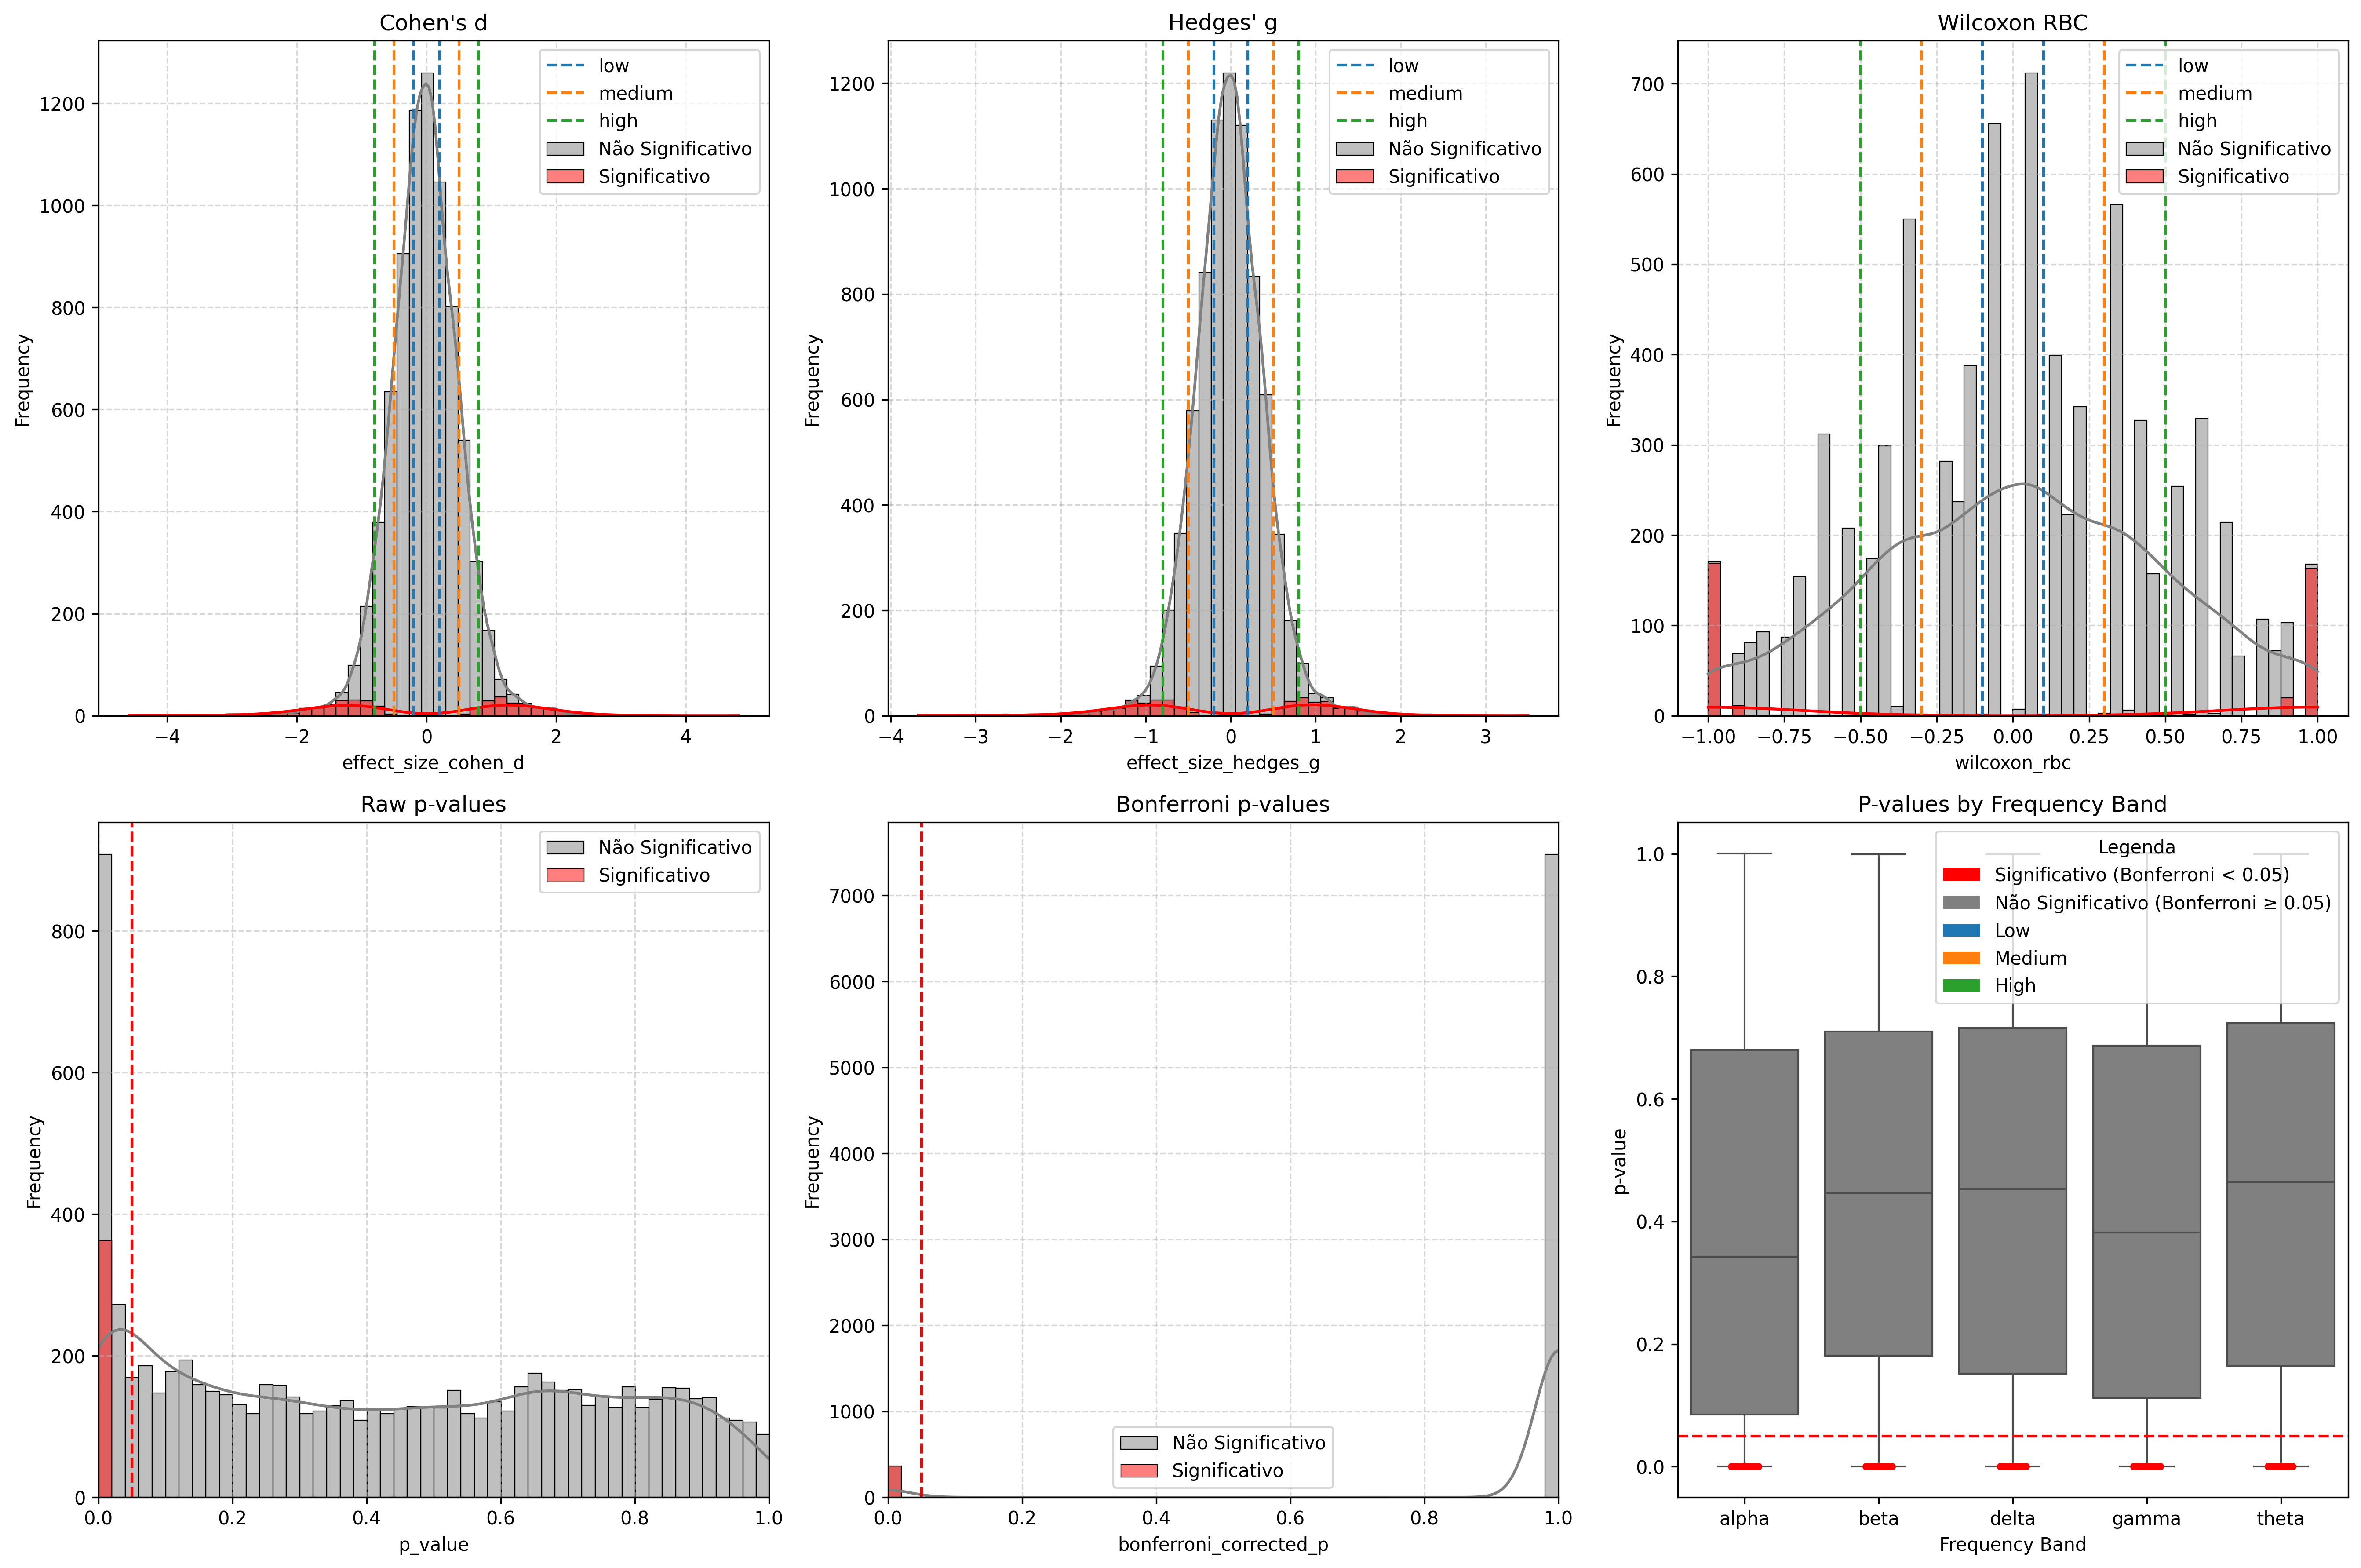
\includegraphics[width=0.45\textwidth]{figs/7_bootstrap_results_analysis/1_effect_size_histograms/Effect_Size_Histograms_PLI_EEGEEG_Sem_Outliers.png}
    }
    \quad
    % Subfigura 2: CF-PLM (EEG-ECG), Sem Outliers
    \subfloat[Sem Outliers -- CF-PLM (EEG-ECG)]{
        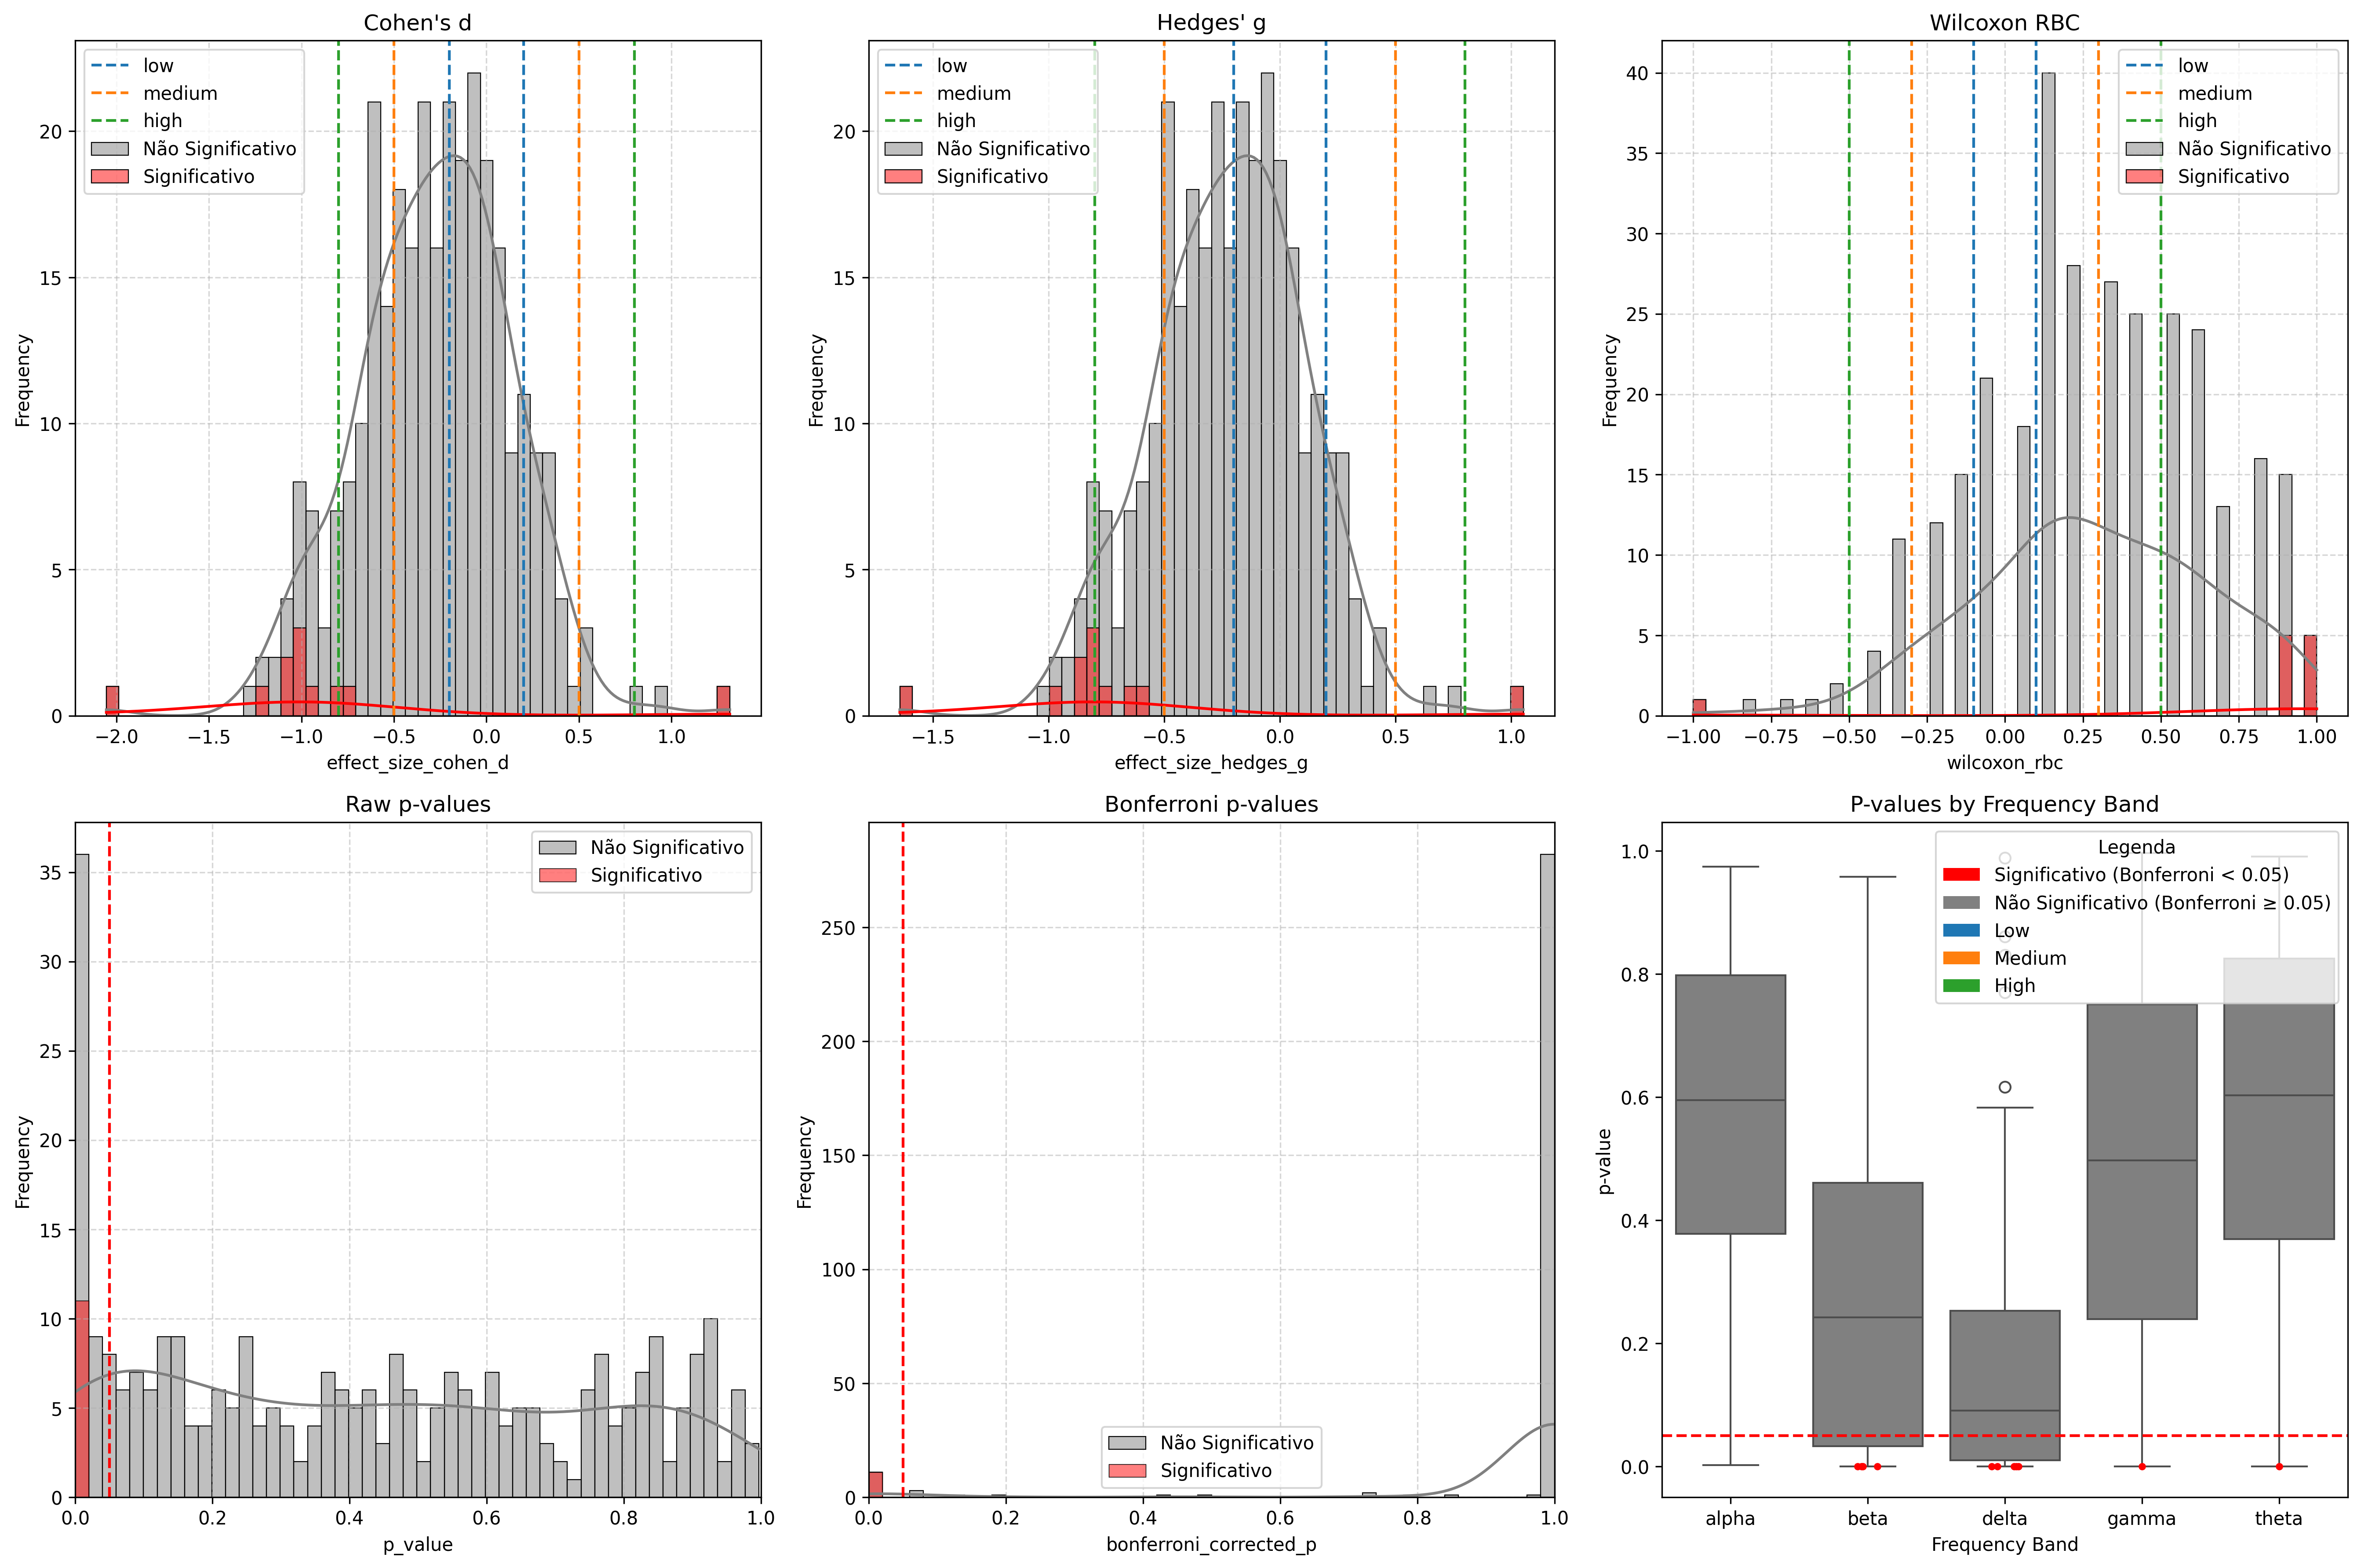
\includegraphics[width=0.45\textwidth]{figs/7_bootstrap_results_analysis/1_effect_size_histograms/Effect_Size_Histograms_CFPLM_EEGECG_Sem_Outliers.png}
    }
    \\
    % Subfigura 3: PLI (EEG-EEG), Com Outliers
    \subfloat[Com Outliers -- PLI (EEG-EEG)]{
        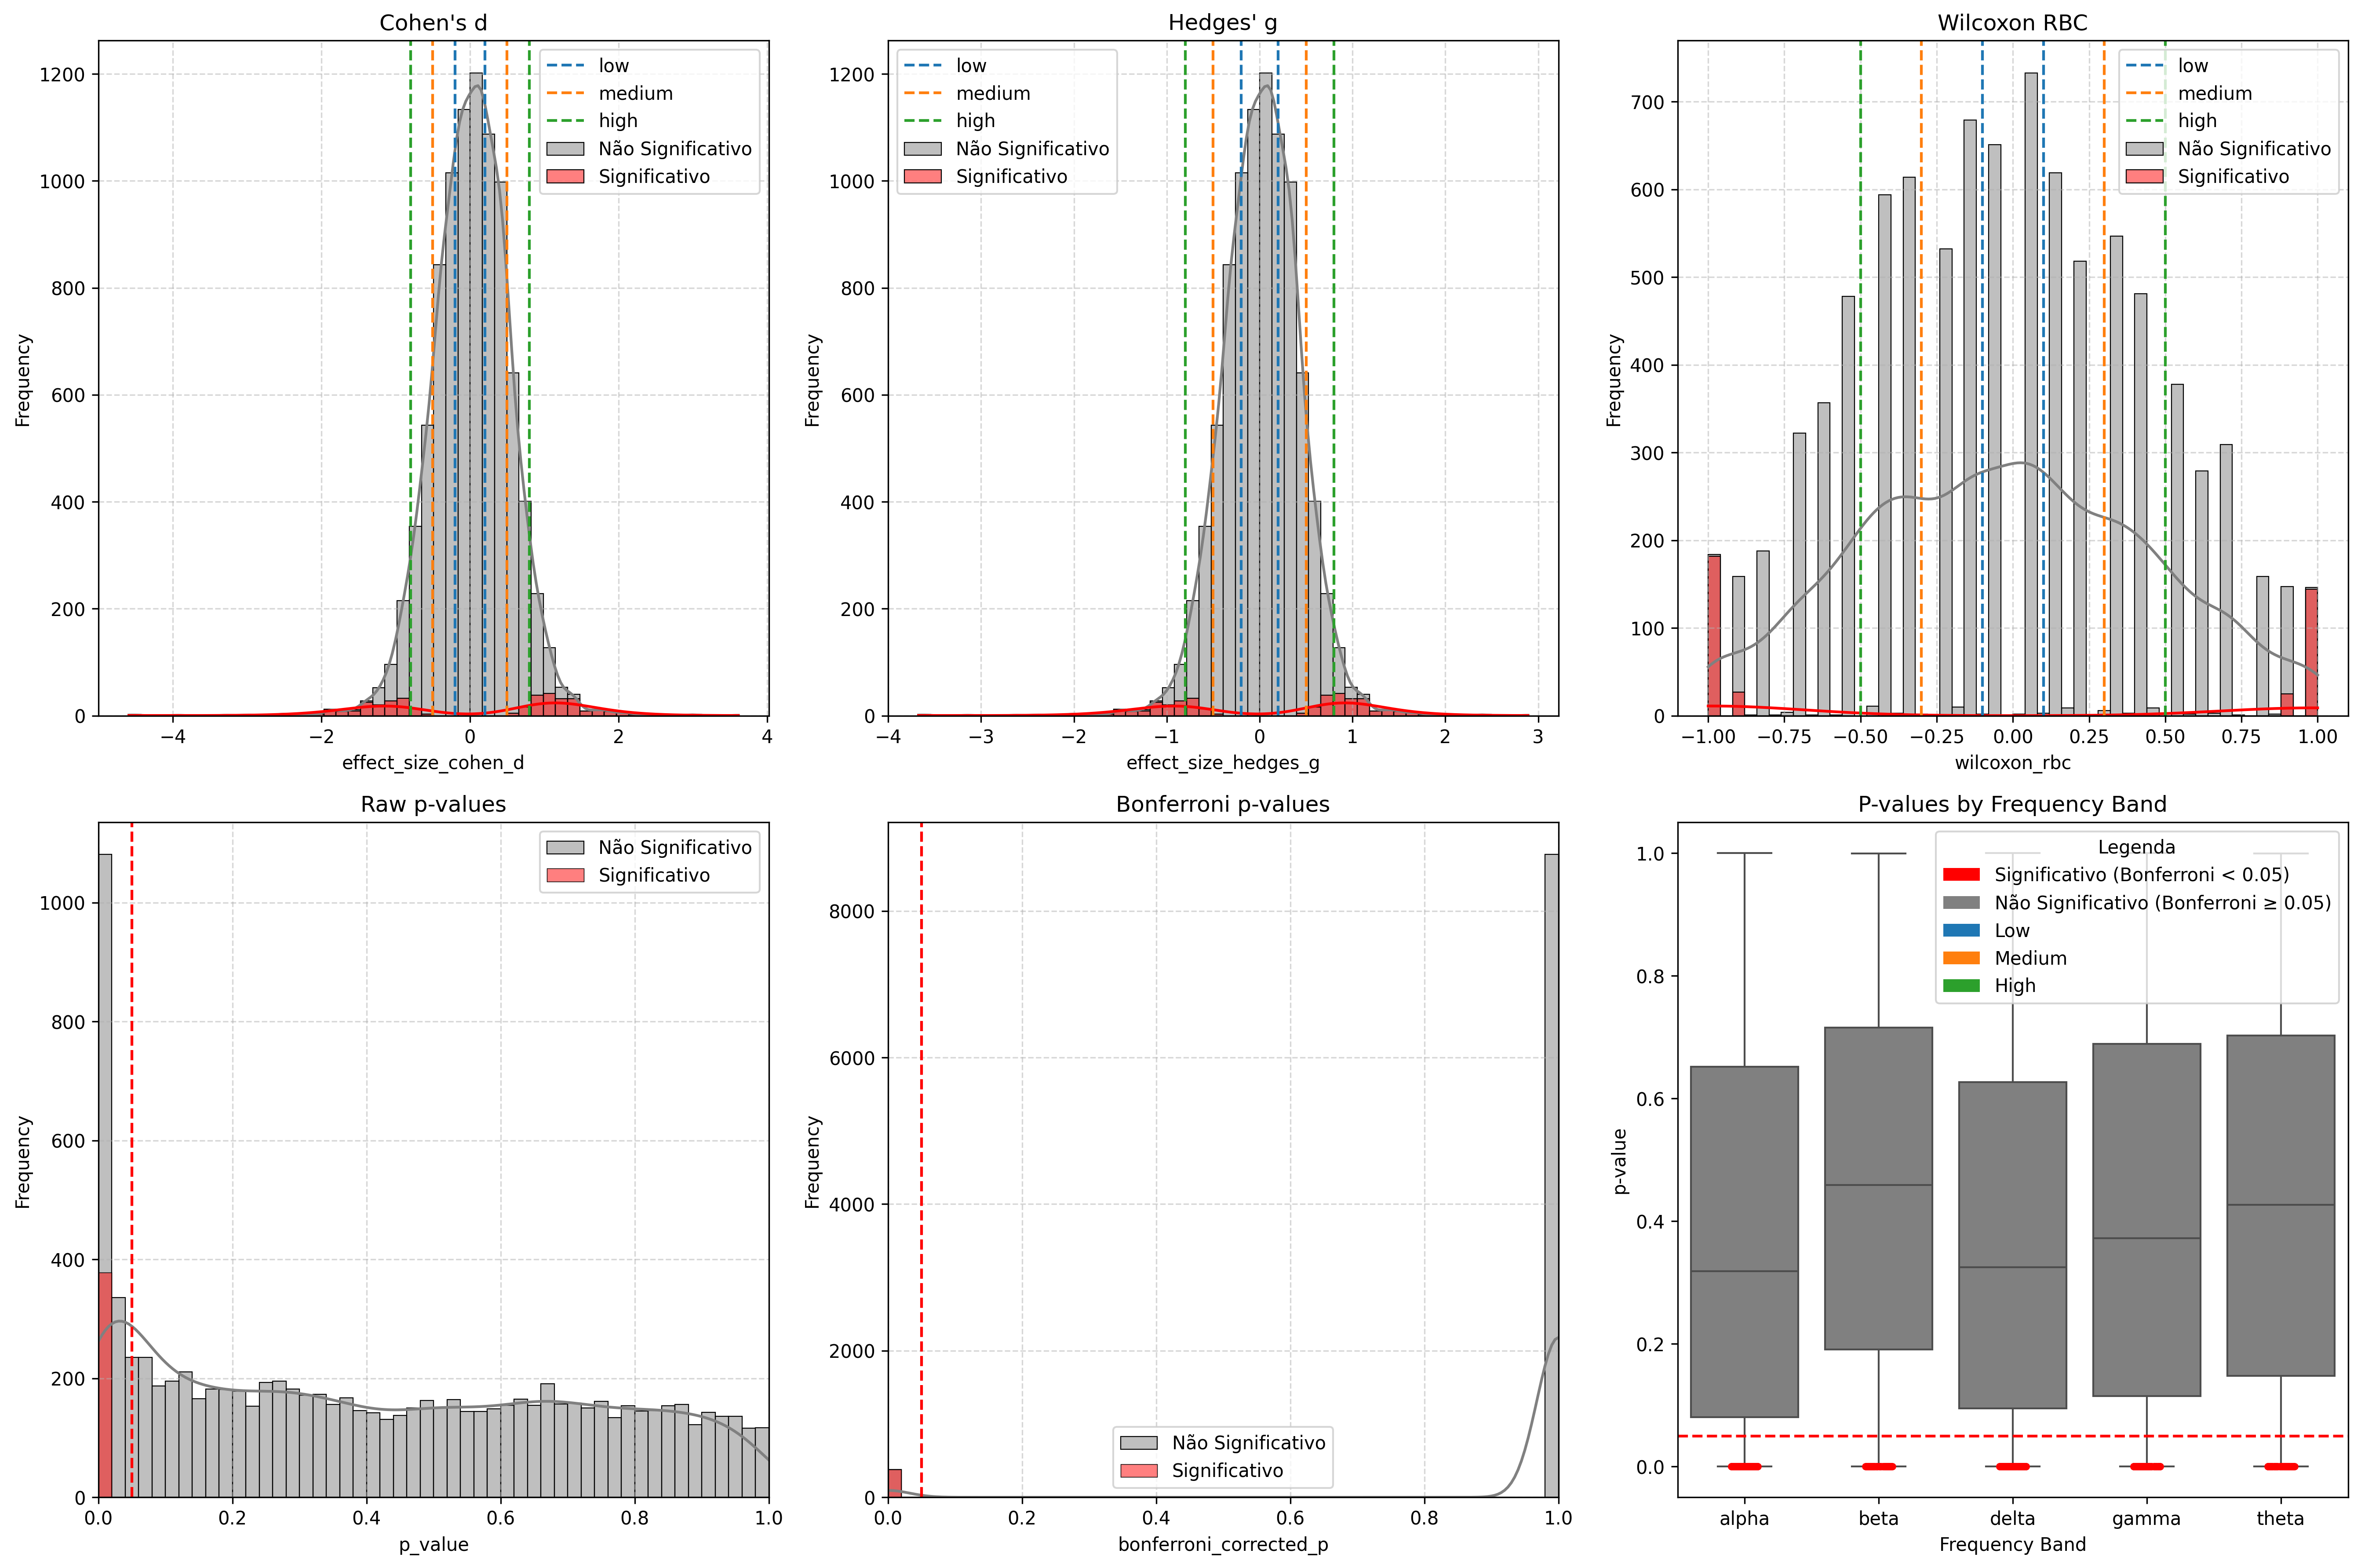
\includegraphics[width=0.45\textwidth]{figs/7_bootstrap_results_analysis/1_effect_size_histograms/Effect_Size_Histograms_PLI_EEGEEG_Com_Outliers.png}
    }
    \quad
    % Subfigura 4: CF-PLM (EEG-ECG), Com Outliers
    \subfloat[Com Outliers -- CF-PLM (EEG-ECG)]{
        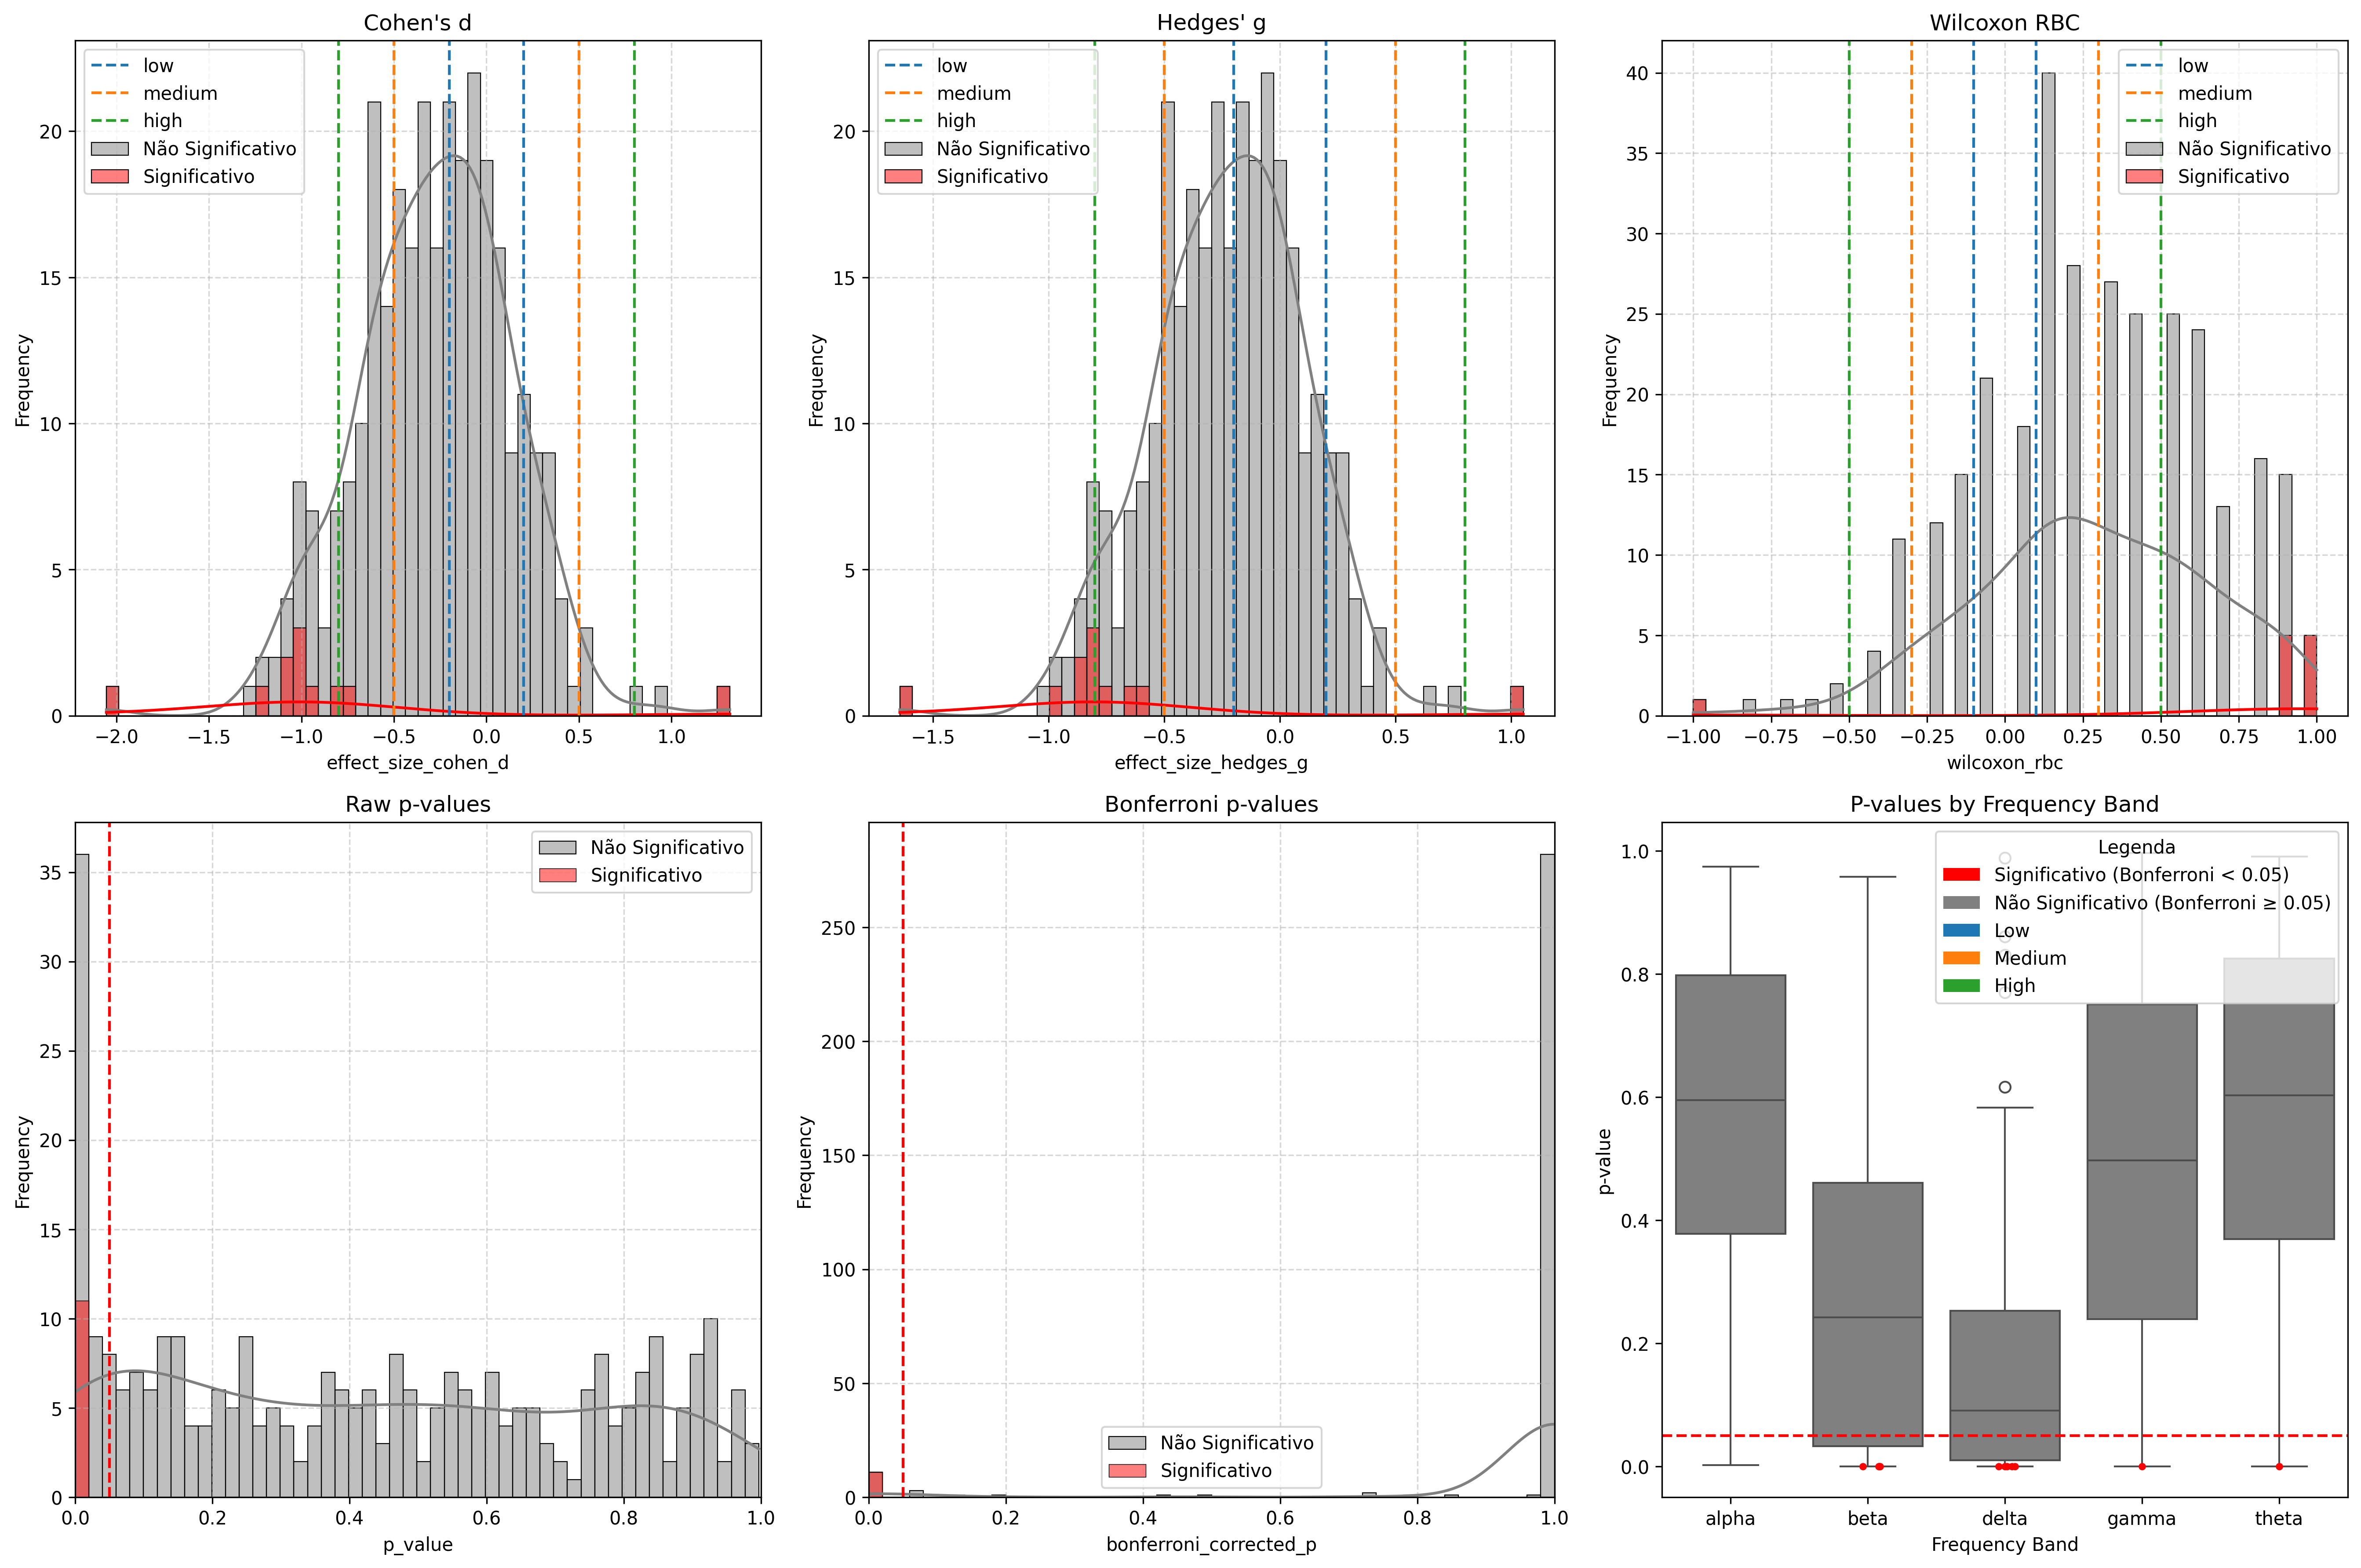
\includegraphics[width=0.45\textwidth]{figs/7_bootstrap_results_analysis/1_effect_size_histograms/Effect_Size_Histograms_CFPLM_EEGECG_Com_Outliers.png}
    }
    \caption[Distribuições de tamanhos de efeito e valores-p]{Distribuição das métricas de tamanho de efeito (\emph{Cohen's d}, \emph{Hedges' g} e \emph{Wilcoxon RBC}) e dos valores-p (brutos e corrigidos por Bonferroni) para PLI (EEG-EEG) e CF-PLM (EEG-ECG), em cenários com e sem outliers. O \emph{Wilcoxon RBC} e o p-valor corrigido por Bonferroni (vertical tracejada vermelha em $p=0.05$) são enfatizados como as métricas mais robustas para, respectivamente, o tamanho de efeito e a significância estatística.}
    \label{fig:effectsizehist_all}
\end{figure}

\subsection{Distribuição dos Tamanhos de Efeito}

\paragraph{Cohen's d e Hedges' g}
\begin{itemize}
    \item A maior parte dos valores concentra-se em torno de zero, indicando que, para a maioria dos pares, as diferenças entre \emph{cathodic} e \emph{sham} são pequenas ou não significativas.
    \item Valores significativos (barras vermelhas nos histogramas) tendem a se afastar de zero, sinalizando diferenças mais acentuadas. Por exemplo, \emph{Cohen's d} ou \emph{Hedges' g} acima de 0.5 (ou abaixo de -0.5) sugere um efeito moderado, e acima de 0.8 (ou abaixo de -0.8) indica um efeito alto.
    \item \emph{Hedges' g} difere de \emph{Cohen's d} por aplicar uma correção para tamanhos amostrais pequenos, mas ambas exibem comportamentos semelhantes nos histogramas.
\end{itemize}

\paragraph{Wilcoxon RBC (Rank-Biserial Correlation)}
\begin{itemize}
    \item O \emph{Wilcoxon RBC} é derivado do teste não paramétrico de Wilcoxon, refletindo a correlação de postos entre as condições (tipicamente variando de -1 a +1).
    \item Por não exigir pressupostos de normalidade, o RBC mostra-se mais robusto ao lidar com dados heterogêneos e eventuais outliers. 
    \item Valores acima de 0.3 ou abaixo de -0.3 sugerem efeito moderado; acima de 0.5 (ou abaixo de -0.5) indicam efeito alto. Quando se aproxima de ±1, as condições diferem de forma quase absoluta.
    \item Devido a essa robustez, o RBC será nosso principal indicador de tamanho de efeito nas análises subsequentes.
\end{itemize}


\subsection{Distribuição de p-valores (Brutos e Corrigidos)}

\begin{itemize}
    \item Os histogramas de valores-p brutos exibem forte concentração em torno de 1 (resultados não significativos) e uma cauda próxima de 0 (potenciais resultados significativos).
    \item Após a correção de Bonferroni (marcada pela linha vertical tracejada em $p=0.05$), muitos valores que eram marginalmente significativos são deslocados para a região de não significância, evidenciando o caráter conservador desta correção.
    \item Em virtude do elevado número de comparações, a adoção de um método rigoroso como o Bonferroni minimiza a probabilidade de falsos positivos. Por esse motivo, utilizamos o p-valor corrigido por Bonferroni como critério principal de significância.
\end{itemize}


\subsection{Comparação Entre Cenários (Com e Sem Outliers)}
\begin{itemize}
    \item \textbf{Diferenças Mínimas:} De modo geral, a remoção de outliers reduz ligeiramente o número de casos significativos em EEG-EEG, mas não afeta substancialmente a distribuição dos tamanhos de efeito ou dos valores-p. No EEG-ECG, a diferença entre manter ou remover outliers é praticamente irrelevante.

    \item \textbf{PLI (EEG-EEG):} Com um número muito maior de pares (cada um dos 61 canais de EEG formando pares entre si), foram encontrados entre 363 (com remoção de outliers) e 378 casos (sem remoção de outliers) significativos.

    \item \textbf{CF-PLM (EEG-ECG):} Em contraste, apenas 11 casos significativos foram observados, mas aqui cada canal de EEG forma par com o único canal de ECG, resultando em um total menor de pares possíveis.
    
    \item \textbf{Robustez do RBC e do Bonferroni:} Independente de manter ou remover outliers, as comparações que exibem valores elevados de \emph{Wilcoxon RBC} e p-valores corrigidos abaixo de 0.05 permanecem confiáveis. Isso reforça o valor dessas duas métricas (RBC e Bonferroni) na interpretação dos resultados.
\end{itemize}


Em síntese, os histogramas de \emph{Wilcoxon RBC} (tamanho de efeito) e p-valores corrigidos por Bonferroni (significância estatística) demonstram claramente quais pares de canais se destacam por apresentarem diferenças robustas entre \emph{cathodic} e \emph{sham}. Embora \emph{Cohen's d} e \emph{Hedges' g} também sejam úteis para quantificar a magnitude do efeito, nossa análise dá ênfase ao RBC, que é não paramétrico e resiliente à heterogeneidade dos dados. Assim, estes resultados embasam as análises topográficas e de rede apresentadas nas seções seguintes.

\subsection{Conclusões Principais}
\begin{itemize}
    \item A maior parte dos dados concentra-se em torno de zero para todas as métricas, refletindo pequenas diferenças entre as condições, o que é coerente com métodos robustos de correção múltipla (p.\,ex.\ Bonferroni) e o grande número de comparações.
    \item Quando há significância estatística, os tamanhos de efeito se afastam notavelmente de zero (\emph{Cohen's d}, \emph{Hedges' g} ou RBC), sugerindo diferenças substanciais e possivelmente relevantes do ponto de vista neurofisiológico.
    \item O \emph{Wilcoxon RBC} se mostra particularmente robusto para capturar a direção e a magnitude das diferenças sem pressupor normalidade, razão pela qual será enfatizado nas próximas análises topográficas e de grafos de conectividade.
\end{itemize}

Assim, a análise dos histogramas de tamanho de efeito e valores-p fornece um panorama inicial: embora haja muitos casos não significativos, uma fração não desprezível apresenta efeitos moderados ou altos e valores-p corrigidos abaixo do limiar. Tais resultados embasam investigações posteriores, que buscarão caracterizar a localização e as faixas de frequência onde a \emph{neuromodulação} exerce impacto mais pronunciado.


\section{Análise de Rede para PLI (EEG-EEG)}
\label{sec:rede_pli_eeg}

Nesta seção, analisamos as redes de conexões significativas obtidas pela métrica PLI para pares EEG-EEG, segmentadas por bandas de frequência, considerando os cenários com e sem outliers. Cada nó representa um canal EEG, e o número ao lado indica o total de conexões significativas envolvendo esse canal. Linhas vermelhas representam conexões com valores de \emph{Wilcoxon RBC} tendendo a +1, indicando conexões robustas.

Apresentamos aqui apenas exemplos representativos das redes (por exemplo, banda Alpha), enquanto a análise completa, contemplando todas as bandas e cenários, pode ser encontrada no \textbf{Apêndice \ref{apendice:pli_eeg_eeg}}.

\begin{figure}[htb]
  \centering
  \includegraphics[width=0.75\textwidth]{figs/7_bootstrap_results_analysis/2_network_graphs/PLI_EEG-EEG_Sem_Outliers/Banda_Alpha_(8_Hz_a_13_Hz)_-_Análise_de_Rede_-_PLI_EEG-EEG_Sem_Outliers.png}
  \caption{Exemplo da rede de conexões significativas na banda Alpha (8--13\,Hz) para PLI (EEG-EEG) no cenário sem outliers. Observa-se um núcleo central de canais altamente conectados, sugerindo forte sincronização.}
  \label{fig:exemplo_rede_pli_alpha_sem}
\end{figure}

\subsection{Resumo das Comparações (PLI EEG-EEG)}

A comparação detalhada entre os cenários com e sem outliers revela que:

\begin{itemize}
    \item A \textbf{topologia das redes permanece semelhante entre os cenários}, indicando que a métrica PLI é robusta mesmo após a remoção de outliers.
    \item A remoção de outliers resulta em uma \textbf{leve redução no número de conexões significativas}, mas \textbf{não altera substancialmente a estrutura da rede}.
    \item Os \textbf{canais com maior centralidade são consistentes} em ambos os cenários, reforçando a confiabilidade dos achados.
\end{itemize}

Para uma análise detalhada de todas as bandas de frequência e cenários, consulte o \textbf{Apêndice \ref{apendice:pli_eeg_eeg}}.

\section{Análise de Rede para CF-PLM (EEG-ECG, Cross-frequency)}
\label{sec:rede_cfplm_eeg_ecg}

Nesta seção, avaliamos as redes de conectividade \textbf{cross-frequency} entre EEG e ECG usando a métrica CF-PLM. Como os resultados mostram um padrão relativamente estável entre os cenários analisados, apresentamos aqui apenas um \textbf{exemplo representativo} (banda Beta). A análise completa para todas as bandas pode ser encontrada no \textbf{Apêndice \ref{apendice:cfplm_eeg_ecg}}.

\begin{figure}[htb]
  \centering
  \includegraphics[width=0.75\textwidth]{figs/7_bootstrap_results_analysis/2_network_graphs/CF-PLM_EEG-ECG_Sem_Outliers/Banda_Beta_(13_Hz_a_30_Hz)_-_Análise_de_Rede_-_CF-PLM_EEG-ECG_Sem_Outliers.png}
  \caption{Exemplo da rede CF-PLM na banda Beta (13--30\,Hz) para EEG-ECG sem outliers. Apesar da rede ser relativamente esparsa, os pares significativos indicam uma sincronização robusta.}
  \label{fig:exemplo_rede_cfplm_beta_sem}
\end{figure}

\subsection{Resumo das Comparações (CF-PLM EEG-ECG)}

As comparações entre os cenários com e sem outliers evidenciam que:

\begin{itemize}
    \item A \textbf{topologia e a quantidade de pares significativos permanecem inalteradas} nos dois cenários, indicando \textbf{independência dos resultados em relação à presença de outliers}.
    \item O \textbf{número total de pares significativos é idêntico (11 casos)}, o que sugere que os efeitos cross-frequency detectados são altamente robustos.
    \item Todos os pares significativos apresentam \textbf{\emph{Wilcoxon RBC} = +1}, reforçando a \textbf{consistência dos achados}.
\end{itemize}

Para mais detalhes e visualização completa das redes de conectividade, consulte o \textbf{Apêndice \ref{apendice:cfplm_eeg_ecg}}.
